% -*- coding: UTF-8 -*-
\documentclass{article}
\usepackage{amsmath}
\usepackage{tikz}

\begin{document}
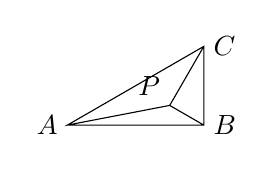
\begin{tikzpicture}

  \coordinate[label=180:$A$] (a) at ({-sqrt(3)},-0.5);
  \coordinate[label=0:$B$] (b) at (0,-0.5);
  \coordinate[label=0:$C$] (c) at (0,0.5);
  \coordinate[label=150:$P$] (p) at (210:0.5);

  \draw (a) -- (b) -- (c) -- (a) -- (p) -- (b) (p) -- (c);

\end{tikzpicture}
\end{document}
